\chapter{医疗知识构建与问答}

任务二以任务一产出的清洗数据集为输入，
经过记录解析、实体关系抽取、校验去重和图谱持久化，
生成可查询的医疗知识图谱，并同步刷新面向分析查询的派生表。
智能体同时绑定建图工具和查询工具，
用户可以在一次对话中完成从数据集到图谱查询的完整流程。

\section{参考知识与增量数据接入}

图谱的基础知识层由两个外部数据源和一个内部质检参考共同构成，
通过 \repoPath{kg/build\_kg\_v2.py} 统一写入 SQLite。

\textbf{QASystemOnMedicalKG（图谱主体）。}
这是一个开源中文医学知识图谱项目~\cite{qasystemkg}，
其核心文件 \texttt{medical.json} 以 JSONL 格式收录了 14\,408 种疾病的结构化信息，
每种疾病携带症状、药物、检查、科室、并发症、病因、预防等字段。
构建脚本逐行解析后，按字段到关系的映射表
（如 \texttt{symptom}→临床表现、\texttt{recommand\_drug}→药物治疗、
\texttt{check}→检查、\texttt{cure\_department}→就诊科室）
将每条字段值拆分为三元组写入图谱，
贡献 420\,221 条三元组。
写入过程中对症状字段执行质量检查：
以从 CMeEE 标注数据中提取的症状词汇表为参照，
筛除不包含典型症状字眼且不在词汇表中的条目
（如人名、乱码、数据污染），
被筛除的条目写入质量记录表而不进入图谱。

\textbf{CMeIE 标注数据（关系补充）。}
CMeIE 是 CBLUE 基准中的中文医学信息抽取数据集~\cite{cblue2022}，
包含 14\,339 条已标注实体和关系的句子。
构建脚本将标注的实体对和关系类型
通过 \texttt{CMEIE\_RELATION\_MAP} 映射为项目的 15 类标准关系后入库，
贡献 25\,046 条三元组。
此外，CMeIE 定义的 43 种关系类型和实体类型体系
也是后续抽取校验模块中类型合法性的判断依据
（\repoPath{core/medical\_extraction\_validation.py} 的 \texttt{ENTITY\_TYPES} 和 \texttt{CMEIE\_RELATION\_TYPES}）。

\textbf{CMeEE 标注数据（质检词典）。}
CMeEE 同样是 CBLUE 的标注数据，用于实体识别评测。
在离线构建阶段，构建脚本从中提取全部已标注的症状实体，
形成一份“确认是症状”的词汇表，
用于过滤 \texttt{medical.json} 中质量存疑的症状字段。
CMeEE 本身不直接导入图谱，
而是作为质检参考标准参与基础知识层的质量把关。

三者的分工是：
QASystemOnMedicalKG 提供覆盖面，CMeIE 提供标注精度，
CMeEE 提供质检依据。
基础构建程序还定义了 15 类标准关系，
以关系代码和中文显示名分开保存，
使不同数据来源中的“临床表现”“相关症状”等表达归并到统一查询口径。

基础知识层构建完成后，
任务一交付数据集进入任务二处理流程时，
每次处理都注册独立来源，
新增事实沿用同一套实体、关系和三元组表结构，
增量数据与基础知识共用同一查询和分析入口。当前在线实例中，
增量管道累计贡献 553 条三元组，
作为独立来源（DataMate 增量）与基础知识共存于同一统计口径。

\section{统一医疗记录解析}

任务二处理流程的第一步是将 DataMate 数据集中的清洗后文件转换为统一的记录流。
共享解析模块按文件扩展名和内容类型分派处理：
TXT 以空段落切分，单段超过 1\,200 字符时按句号边界继续拆分；
CSV 经 \texttt{csv.DictReader} 逐行序列化，保留列名作为字段键；
JSON 数组逐项生成记录，对象整体作为一条；
JSONL 按非空行逐条解析。
每条记录统一携带 \texttt{record\_id}、
\texttt{source\_file}、\texttt{source\_format} 和原始字段；
结构化记录原本带有 \texttt{record\_id} 或 \texttt{id} 时，另存为
\texttt{source\_record\_id}，否则使用源文件名加行号或分段号生成稳定记录号，
确保下游抽取模块无需区分原文件的物理格式。

当用户通过 \texttt{max\_records} 参数限制单次处理量时，
选择模块采用跨文件轮转抽样：按源文件分桶后轮流从各桶取一条，
使处理额度在各文件之间均匀分配。
例如 5 个文件各 100 条记录、限制 50 条时，
每个文件贡献 10 条。

\begin{figure}[H]
\centering
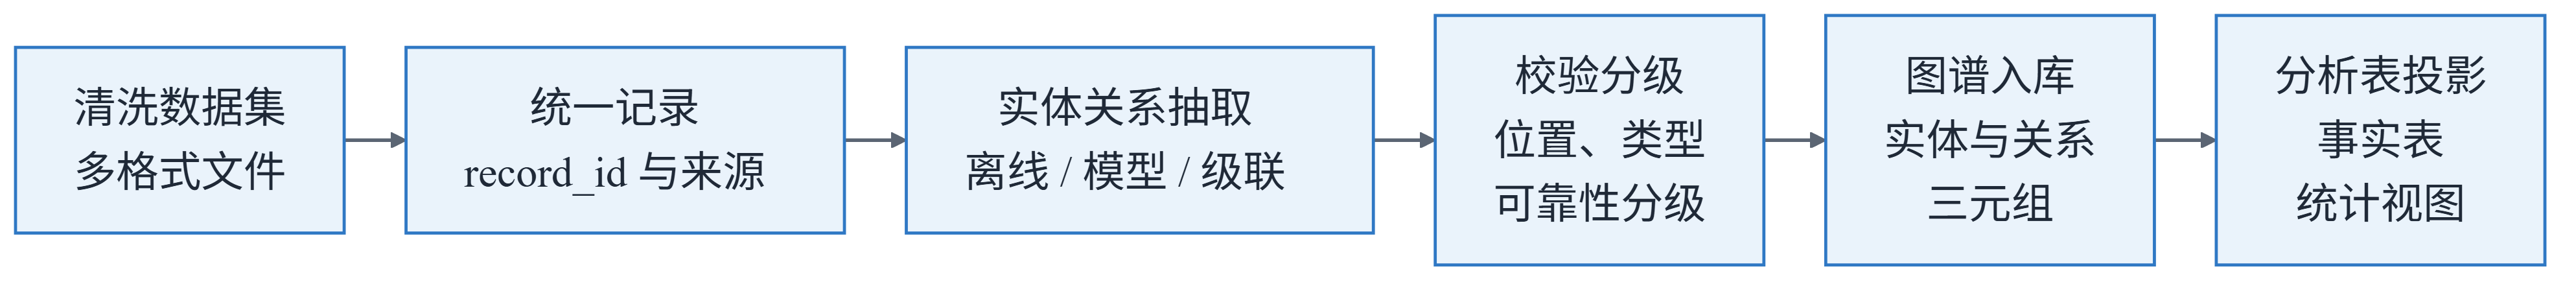
\includegraphics[width=0.98\textwidth]{figures/mermaid_kg_pipeline.png}
\caption{清洗数据集到知识图谱和分析表的处理流程}
\label{fig:task2-pipeline}
\end{figure}

\section{实体关系级联抽取}

统一抽取服务提供三种可切换的后端。

任务二的 DataMate 算子把记录处理拆成可注册的单步处理。
表~\ref{tab:task2-operators} 给出算子接口与在线建图服务的对应关系。

\begin{table}[H]
\centering
\small
\caption{任务二算子接口与处理结果}
\label{tab:task2-operators}
\begin{tabularx}{\textwidth}{L{3.1cm}L{4.8cm}Y}
\toprule
\textbf{算子} & \textbf{输入与处理} & \textbf{输出字段} \\
\midrule
\makecell[l]{MedicalEntity\\Extractor} &
读取记录文本，按离线、模型或混合后端识别九类医疗实体 &
\texttt{entities}、后端标识和抽取耗时 \\
\addlinespace
\makecell[l]{MedicalRelation\\Extractor} &
结合实体结果抽取疾病与其他实体之间的关系 &
\texttt{relations}、后端标识和抽取耗时 \\
\addlinespace
\makecell[l]{MedicalTriple\\Generator} &
将实体关系转换为三元组，并按可靠性等级分流 &
\texttt{triples}、入库数量和质量记录 \\
\addlinespace
\makecell[l]{MedicalText\\QualityFilter} &
检查医疗文本长度、特殊字符比例和重复内容 &
质量状态、过滤原因和处理统计 \\
\bottomrule
\end{tabularx}
\end{table}

上述算子以 \texttt{operators/*/process.py} 和 \texttt{metadata.yml} 作为可部署资产。
在线建图入口读取 DataMate 数据集后，
由 \texttt{core/medical\_extraction\_service.py} 选择抽取后端，
再由任务二服务完成校验、事务写入和分析库刷新。
算子接口和在线服务共享抽取模型与校验逻辑，
调用入口分别面向 DataMate 任务和数据集级 MCP 工具。

对于用户在 Nexent 中直接给出或要求生成的一段医疗文本，智能体调用统一文本抽取工具
（\texttt{extract\allowbreak\_medical\allowbreak\_knowledge\allowbreak\_from\allowbreak\_text}）。
该入口只运行一次抽取链，同时返回
\texttt{entities}、\texttt{relations}、\texttt{triples}、
\texttt{cascade}、\texttt{performance} 和 \texttt{extraction\_errors}。
返回空数组表示该段文字未识别到相应事实，仍属于结构完整的成功结果；
三个拆分入口保留用于兼容单项调用，但智能体不再把同一文本重复抽取三次。
自拟病历在调用前移除引号并整理为一个纯文本参数，避免对话平台把病历中的引号误判为调用语法边界。

\subsection{离线词典规则抽取}

离线抽取模块实现了不依赖外部模型的抽取链。

\textbf{实体识别}的执行过程为：
第一，加载独立维护的医学词典 \texttt{entity\_lexicon.json}，
当前资产包含约 3.17 万条术语，词条由 CMeEE-V2 和 CMeIE 训练数据整理生成；
运行时再与已有图谱实体合并，统一映射到 CMeEE 的实体类型；
第二，长词优先匹配：先匹配“2型糖尿病”再匹配“糖尿病”，
已占用的字符区间不再被短词覆盖；
第三，过滤停用词（“患者”“医生”“治疗”等通用词）、
纯数字串、长度小于 2 或大于 32 的字符串；
第四，为每个命中位置截取前后各 20 个字符作为原文片段。

\textbf{关系抽取}以疾病为中心，但不再把句内共现直接视为事实。
模块先在同一句或受限文本窗口内定位疾病与其他实体，
优先复用图谱和 CMeIE 资产中已经出现过的主客体关系；
没有已知关系时，必须同时满足实体类型约束和关系触发词，
例如“表现为”支持临床表现，“位于、累及”支持发病部位，
“由于、导致”支持病因，“给予、服用”支持药物治疗。
仅有实体共现、没有对应触发证据的候选不会直接形成关系。
对于 CMeIE 常见的“疾病@正文”结构，标题疾病会在同一分段的后续句中继承，
使检查、部位和病因等关系仍有明确主语；遇到新的疾病标题时立即切换归属。
普通病历还识别“初步诊断、入院诊断、出院诊断”等明确诊断句：
诊断后的三句、360 个字符以内，给药、实施治疗和并发症枚举可以继承最近的首个诊断疾病；
跨空段或遇到新的诊断句即停止继承。该窗口只解决“诊断在前一句、处理在后一句”的病历写法，
不把整段任意共现实体相互连接。
最后，\texttt{NEGATION\_RE} 检查“无”“未见”“否认”“排除”等否定表达，
命中否定范围的实体不生成关系。

\subsection{模型补充抽取}

\texttt{core/medical\_ner.py} 和 \texttt{core/medical\_re.py}
将医疗记录组织为结构化抽取请求，
要求模型返回实体（文本、类型缩写、起止位置）和关系（头尾实体、关系类型），
均为 JSON 数组格式。
模型返回的结果随后经过与离线方式相同的校验和去重管道。

\subsection{离线优先级联抽取}

\texttt{hybrid}（混合方式）采用离线优先的级联流程，
先扫描全文，再根据句子覆盖情况和候选可靠性决定模型的使用范围。
离线方式和混合方式的第一阶段调用同一套词典、关系规则和质量门禁。
句子覆盖情况由句内已识别实体、关系以及医疗提示词共同判断：
若存在未参与关系的实体、关系类型缺失或因果、部位等提示词未得到对应关系，
该句进入待补充集合；没有这些情况的句子直接进入统一校验。
高、中可靠离线候选直接保留；低可靠实体进入 LLM 复核；
低可靠关系只放行两类窄候选：历史分组精确率达到路由条件且带原文触发词的候选，
以及“明确给药句、明确诊断后续句”产生并已通过确定性证据检查的候选；
旧的泛句内共现和全文上下文候选仍被门禁拦截；
离线链路未覆盖但包含医疗提示词的句子进入模型补充，
模型只能返回原文直接支持的实体和关系。
图~\ref{fig:task2-cascade} 展示了这条处理路径。

\begin{figure}[H]
\centering
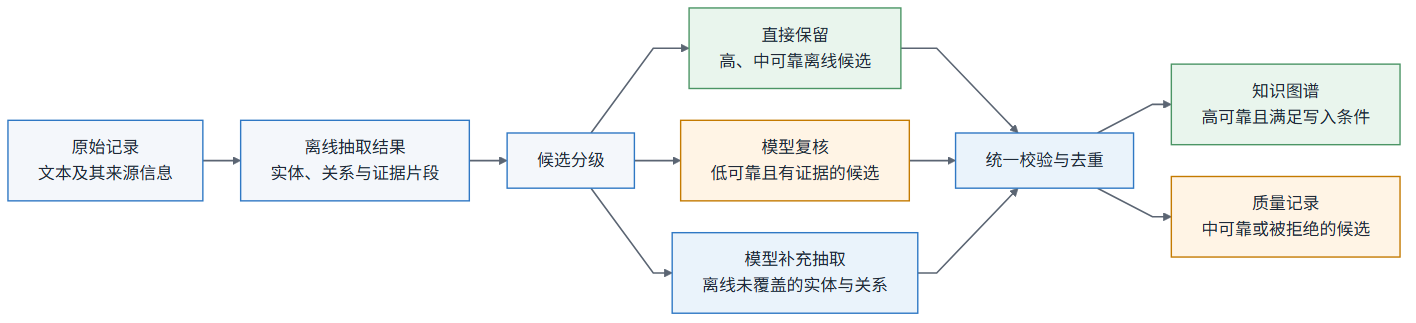
\includegraphics[width=0.98\textwidth]{figures/mermaid_cascade.png}
\caption{离线优先的实体关系级联抽取流程}
\label{fig:task2-cascade}
\end{figure}

级联流程由任务二服务负责编排。服务根据句子内实体和关系覆盖情况筛选待补充句，并限制一次模型补充的句子数量；模型调用只返回原文直接支持的实体和关系。模型补漏实体与复核恢复的低可靠离线实体共用同一套规范化门禁，统一检查原文边界、完整词形、实体类型、否定范围和噪声片段。实体的起止位置必须与原文切片逐字相等，例如原文只有“胸痛”时，“胸痛（术后）”不能通过；新增关系还必须通过端点存在性、关系类型和触发词证据校验。高分且属于已校准安全类型的候选可以直接进入合并，其余候选再与低可靠离线候选一起复核。
复核通过的新增事实标记为高可靠，
抽取方式字段写入 \texttt{llm\allowbreak\_gap\allowbreak\_verified}。
其两个端点也必须通过实体校验；
缺失、拒绝或不确定的决定不会新增事实。

批量处理分两阶段完成：
第一阶段逐条执行离线抽取，并为每条记录加上独立候选范围；
第二阶段只对存在待补充句的记录并发调用模型补充，
每批最多使用 4 个工作线程，单条调用超时后保留该记录的离线结果。
待补充关系、低可靠离线关系、待补充实体和低可靠离线实体按顺序进入复核队列；每一层都按记录轮转抽取候选，避免前部记录占满额度。
队列上限为 256 条；随后调用 \path{review_candidates()} 统一处理。
合并阶段以记录标识限定候选范围，避免批量处理时将其他记录的复核结果错误关联到当前记录。
模型调用失败时，服务保留已经通过离线质量门禁的实体、关系和三元组，
并在处理结果记录的 \texttt{llm\_error} 字段中返回错误信息。
因此，\texttt{hybrid} 在保留离线可复现结果的同时，
只把有原文依据的补充事实交给后续入库流程。

\subsection{基于可靠性分级的事实持久化}

系统从 \texttt{reliability\_profile.json} 读取按处理阶段、抽取方法和实体或关系类型划分的验证结果，
将候选标记为高、中、低三级。配置中的分组精确率用于入库决策，
表示同组方法的历史可靠性，不表示单条事实的概率。

对离线候选，分组可靠性分按
\[
  p_g=\frac{TP_g}{N_g},\qquad
  g=(s,m,c)
\]
计算，其中 (s)、(m)、(c) 分别表示处理阶段、抽取方法和实体或关系类型，
\(N_g\) 是验证集中该组输出数量，\(TP_g\) 是严格命中的数量。
因此，同为“词典精确匹配+疾病”的多个实体会显示相同分数，这是按组校准的结果，不是程序把每条事实都判断成同一概率。
低可靠候选经模型明确接受后，抽取方式改为
\texttt{llm\_review\_verified}，可靠等级提升为高，界面分数改用本次模型裁决返回值；
该值仍是复核信号，不应解释为临床风险概率。

\begin{table}[H]
\centering
\caption{任务二候选事实的可靠性分级}
\label{tab:reliability-tiers}
\begin{tabularx}{0.82\textwidth}{L{2.6cm}L{3.4cm}Y}
\toprule
\textbf{等级} & \textbf{处理方式} & \textbf{写入结果} \\
\midrule
高 & 通过入库校验 & 写入 \texttt{kg\_triples}，保留来源标识、原文片段和抽取方式 \\
中 & 保留为候选 & 写入 \texttt{kg\_quality\_issues}，标记为 \texttt{candidate\_fact} \\
低 & 不进入主图谱 & 写入 \texttt{kg\_quality\_issues}，标记为 \texttt{rejected\_fact} \\
\bottomrule
\end{tabularx}
\end{table}

持久化层遇到缺失的可靠性标记时，将 LLM 结果按中等级处理，
其他来源按低等级处理。这样，只有明确归入高等级的事实进入主图谱，
中、低等级候选都保留在质量记录中，供复核和统计使用。

\subsection{知识构建与问答路由}

知识图谱生成与问答智能体根据用户目标选择不同工具入口。
用户要求处理数据集或重新建图时调用\path{run_task2_kg_pipeline}；
用户给出或要求生成单段医疗文本时调用\path{extract_medical_knowledge_from_text}，一次取得实体、关系、三元组和性能统计；
用户询问疾病属性时调用\path{query_disease_analytics}；
用户要求查看实体关系时调用\path{query_knowledge_graph}；
用户询问已登记来源时调用\path{get_medical_data_sources}。
这些工具共享同一套来源、实体和关系数据，
问答阶段读取的是建图阶段已经提交的事实。

建图工具和任务二服务默认使用 \texttt{hybrid} 后端，
先执行离线全量扫描，再按级联规则调用模型；
需要完全可复现的批量导入时，可以显式指定 \texttt{offline}。
智能体根据工具返回的\texttt{status}、来源文件摘要、生成三元组数量、
入库数量和分析库刷新状态组织回答；
部分记录失败或分析库未刷新时，
回答保留对应状态，并将候选抽取结果与已入库事实分别展示。

\section{实体关系校验与入库}

抽取产生的候选依次经过类型检查、字段归一化、可靠性分级与去重，
再由持久化服务完成数据库去重和写入。前四项检查由
\path{core/medical_extraction_validation.py} 负责，
持久化服务由 \path{mcp_server/kg/persistence.py} 执行最终写入。

\textbf{第一道：类型校验。}
实体类型只接受 9 类（疾病、症状、药物、设备、治疗、身体部位、检查、微生物、科室），
通过 \texttt{ENTITY\_TYPE\_ALIASES} 将中文名、英文名统一映射为内部缩写；
关系类型只接受 CMeIE 标准集中的 43 种，
通过 \texttt{RELATION\_ALIASES} 将“症状”“科室”等常见简称映射为标准名。
实体文本必须在原始记录中能够定位；模型结果给出的起止位置还必须满足
\texttt{text[start:end+1] == entity.text}，位置缺失时只接受原文中唯一的精确出现，
关系中的头尾实体名必须同时出现在原文中。

\textbf{第二道：归一化。}
抽取侧将模型返回的各种写法统一为内部代码
（实体类型“症状”→\texttt{sym}，关系别名“症状”→“临床表现”）；
持久化侧（\path{mcp_server/kg/normalization.py}）再映射为英文关系代码和中文展示名
（“临床表现”→\texttt{has\_symptom}，展示名“临床表现”；
“药物治疗”→\texttt{treated\_by\_drug}，展示名“药物治疗”）。
两层归一化确保离线词典、模型和混合三种抽取方式产出的字段落在同一值域。

\textbf{第三道：可靠性分级与去重。}
实体在校验函数内按出现位置和类型去重，
关系按主语、谓词和宾语去重；
三元组转换步骤再次按同一组合去重，并保留抽取置信度和可靠性等级。通用转换函数默认使用 0.7 的置信度下限；在线级联入口显式保留候选，最终是否进入主图谱由高、中、低三级持久化规则决定。0.7 阈值承担通用转换过滤，三级可靠性承担最终持久化分流。

\textbf{第四道：数据库去重与写入。}
持久化服务按记录逐条写入：先按名称和类型保持实体唯一，
再确保关系类型唯一，最后按主语、关系、宾语、来源标识和原文片段的组合写入三元组。
同一名称在不同实体类型中可以分别保留，
同一事实来自不同文件时各自保留独立来源标识和原文片段。
三元组同时保存 \texttt{source\_file} 和 \texttt{source\_record\_id}，
查询结果可返回来源数据集、文件、记录号、原文证据、抽取方式和可靠等级。

整个抽取和入库过程由任务二服务统一编排。
每条记录独立处理。某条记录的抽取失败不影响其他记录，
某条三元组的写入失败也不回滚已成功入库的部分。
循环结束后统计实体数、关系数、生成三元组数和实际入库数，
并计算平均抽取时延和吞吐量。

\section{图谱事实的分析投影}

图谱写入完成后，分析刷新服务按三元组中的关系类型，
将规范化事实写入面向查询的派生业务表；服务将这一步记为“分析表刷新”。
\texttt{diseases} 保存疾病主表，
\texttt{disease\_facts} 保存全部疾病事实；
症状、药物、科室、并发症、检查、治疗、病因、预防和易感人群
分别进入 9 张关系表。
\texttt{entity\_stats} 与 \texttt{relation\_stats} 保存统计结果，
五个视图提供实体类型、关系类型、高频症状、科室疾病和药物疾病分布。

刷新只在图谱事务提交成功且存在新增三元组时执行，
避免分析表早于图谱更新，或在没有新增事实时重复刷新。
图谱库承担规范化事实和来源追溯，
分析库承担疾病属性查询、分组统计与排序，
图谱库作为事实和来源的规范存储，分析库作为查询和统计的派生存储，
两者承担不同的数据访问职责。

\section{知识图谱查询}

知识图谱生成与问答智能体绑定一个建图工具和四个查询工具。
建图工具（\path{run_task2_kg_pipeline}）接收 DataMate 数据集标识，
按上述管道完成解析、抽取、入库和分析刷新，
返回来源文件、格式分布、实体数、关系数、入库三元组数、
各阶段耗时和吞吐量。
查询工具按疾病名称读取症状、药物、检查、科室等事实，
以实体为中心返回相邻节点与关系，
列出已登记知识源及其记录规模。
用户可以在一次对话中先启动数据集建图，
再通过查询工具查看来源、疾病事实或实体关系。

\section{运行实例数据构成}

当前运行实例包含 14\,408 个疾病条目、79\,605 个实体、
445\,820 条三元组和 445\,210 条疾病事实。
表~\ref{tab:runtime-kg-sources} 按构建方式列出三元组来源，
图~\ref{fig:runtime-relations} 展示数量较多的关系类型。

\begin{table}[H]
\centering
\caption{运行实例三元组构成}
\label{tab:runtime-kg-sources}
\begin{tabularx}{0.82\textwidth}{Y C{3.2cm}}
\toprule
\textbf{构建方式} & \textbf{三元组数量} \\
\midrule
开放医学知识资源结构化导入 & 420\,221 \\
CMeIE 标注关系导入 & 25\,046 \\
DataMate 与任务二增量流程 & 553 \\
\midrule
合计 & 445\,820 \\
\bottomrule
\end{tabularx}
\end{table}

\begin{figure}[H]
\centering
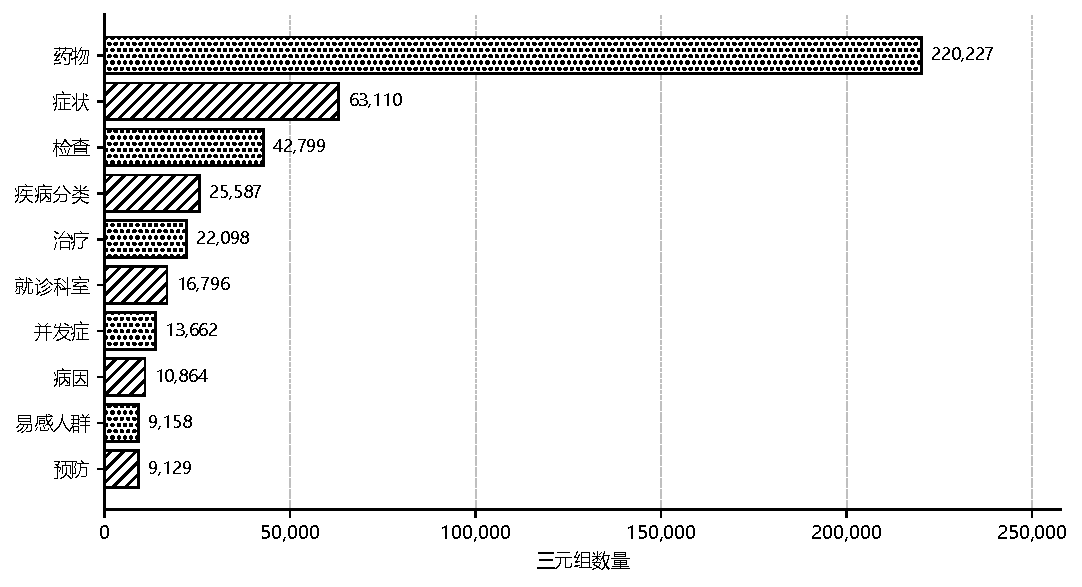
\includegraphics[width=0.88\textwidth]{figures/runtime_relation_distribution.pdf}
\caption{运行实例主要关系类型规模}
\label{fig:runtime-relations}
\end{figure}

运行数据中，药物关系约占全部三元组的一半，
症状、检查、疾病分类和治疗关系的数量居后但仍构成主要关系类别。
DataMate 增量事实作为独立来源进入同一统计口径，
这些来源继续沿用同一组查询工具和分析表。
